% This file was created by matlab2tikz.
%
\documentclass[tikz]{standalone}
\usepackage[T1]{fontenc}
\usepackage[utf8]{inputenc}
\usepackage{pgfplots}
\usepackage{grffile}
\pgfplotsset{compat=newest}
\usetikzlibrary{plotmarks}
\usetikzlibrary{arrows.meta}
\usepgfplotslibrary{patchplots}
\usepackage{amsmath}

\newlength\figureHeight \setlength{\figureHeight}{6cm}
\newlength\figureWidth \setlength{\figureWidth}{10cm}
\begin{document}
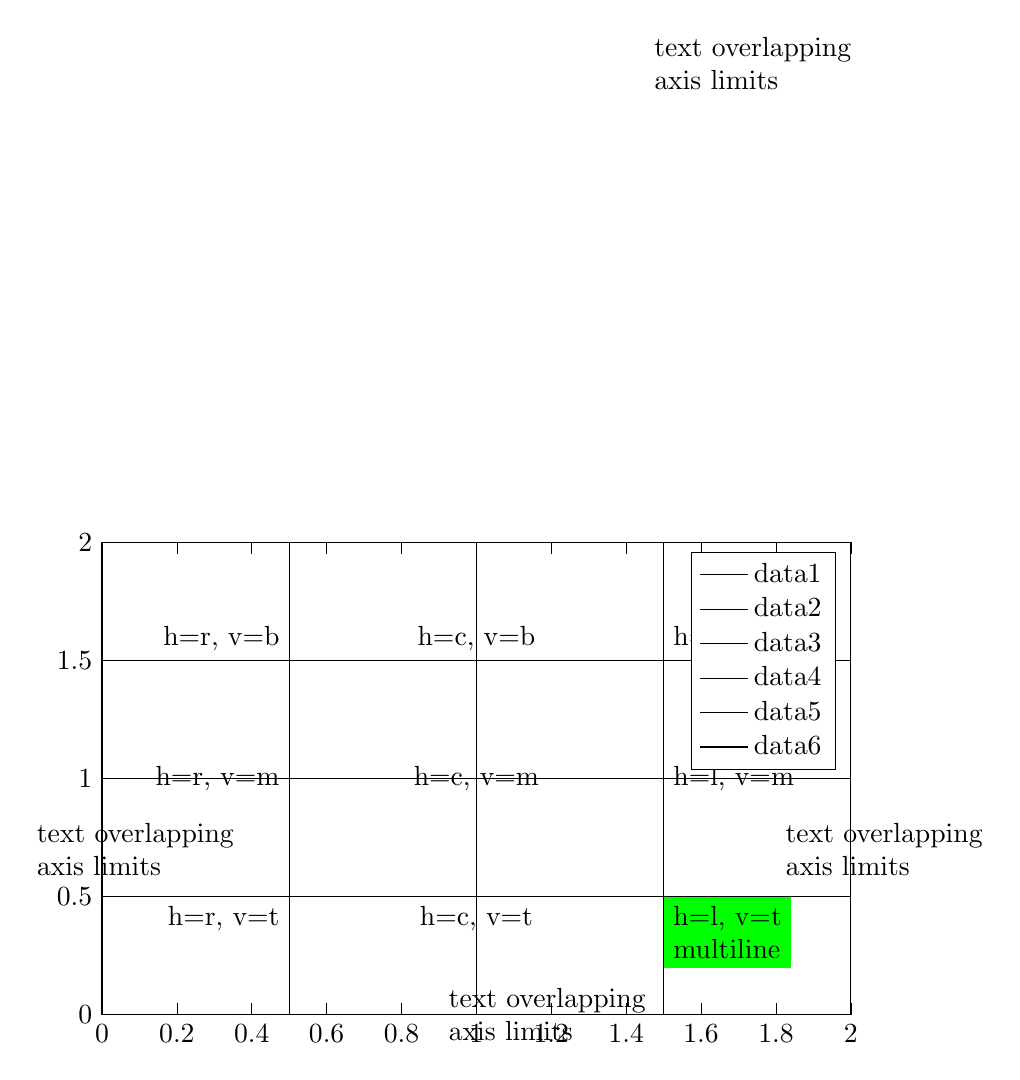
\begin{tikzpicture}

\begin{axis}[%
width=0.951\figureWidth,
height=\figureHeight,
at={(0\figureWidth,0\figureHeight)},
scale only axis,
clip=false,
separate axis lines,
every outer x axis line/.append style={black},
every x tick label/.append style={font=\color{black}},
every x tick/.append style={black},
xmin=   0,
xmax=   2,
every outer y axis line/.append style={black},
every y tick label/.append style={font=\color{black}},
every y tick/.append style={black},
ymin=   0,
ymax=   2,
axis background/.style={fill=white},
legend style={legend cell align=left, align=left, draw=black}
]
\addplot [color=black]
  table[row sep=crcr]{%
   0	   1\\
   2	   1\\
};
\addlegendentry{data1}

\addplot [color=black]
  table[row sep=crcr]{%
   0	 0.5\\
   2	 0.5\\
};
\addlegendentry{data2}

\addplot [color=black]
  table[row sep=crcr]{%
   0	 1.5\\
   2	 1.5\\
};
\addlegendentry{data3}

\addplot [color=black]
  table[row sep=crcr]{%
   1	   0\\
   1	   2\\
};
\addlegendentry{data4}

\addplot [color=black]
  table[row sep=crcr]{%
 1.5	   0\\
 1.5	   2\\
};
\addlegendentry{data5}

\addplot [color=black]
  table[row sep=crcr]{%
 0.5	   0\\
 0.5	   2\\
};
\addlegendentry{data6}

\node[align=center]
at (axis cs:1,1) {h=c, v=m};
\node[right, align=left]
at (axis cs:1.5,1) {h=l, v=m};
\node[left, align=right]
at (axis cs:0.5,1) {h=r, v=m};
\node[above left, align=right]
at (axis cs:0.5,1.5) {h=r, v=b};
\node[above, align=center]
at (axis cs:1,1.5) {h=c, v=b};
\node[above right, align=left]
at (axis cs:1.5,1.5) {h=l, v=b};
\node[below left, align=right]
at (axis cs:0.5,0.5) {h=r, v=t};
\node[below, align=center]
at (axis cs:1,0.5) {h=c, v=t};
\node[fill=green, below right, align=left]
at (axis cs:1.5,0.5) {h=l, v=t\\multiline};
\node[right, align=left]
at (axis cs:1.8,0.7) {text overlapping\\axis limits};
\node[right, align=left]
at (axis cs:-0.2,0.7) {text overlapping\\axis limits};
\node[right, align=left]
at (axis cs:0.9,0) {text overlapping\\axis limits};
\node[right, align=left]
at (6.89cm,12.083cm) {text overlapping\\axis limits};
\end{axis}
\end{tikzpicture}%
\end{document}